%% ch06-ai-synthesis.tex — Chapter VI: Learned Synthesis and Honest Cost Accounting
%% Sources: guo2026rubriq, guo2026rubriqsoftware, guo2026nonlinearwaves, guo2026splitstepqude
%% Label prefix: syn:
%% STE edition: prose edited toward ASD-STE100 (about 80% strictness). Facts, numbers, citations,
%% cross-references, equations, tables, algorithms and the pre-existing figures are unchanged.
\chapter{Learned Synthesis and Honest Cost Accounting}\label{ch:synthesis}

This chapter addresses RQ4: can learned, HPC-scale synthesis produce circuits that respect fault-tolerant resource budgets, and what does honest cost accounting say about end-to-end quantum advantage? Two studies answer the two halves. Both put the full cost of a quantum computation into one programmatic accounting and let it drive the design.

Part~A (\crefrange{sec:syn:prelim}{sec:syn:rubriq-discussion}) presents \rubriq{}: fault-tolerant circuit synthesis as large-language-model (LLM) code generation, fine-tuned by reinforcement learning against a programmatic rubric. \cudaq{} simulation on GPUs evaluates the rubric inside the training loop. Part~B (\cref{sec:syn:waves}) asks what it costs to simulate nonlinear wave equations on a quantum processor when the nonlinearity needs the field itself. Its answer is a unified measurement-and-reload cost model validated on hardware. \Cref{sec:syn:relation} relates both studies to the other chapters, and \cref{sec:syn:summary} summarizes.

\section{Introduction}\label{sec:syn:intro}

The previous chapters scaled simulation (\cref{ch:qgear}), made the classical--quantum data interface vectorized and learnable (\cref{ch:qml}) and replaced black-box variational search with problem structure (\cref{ch:nisq}). Each was measured against today's hardware. This chapter turns to the hardware being built: fault-tolerant processors. Their cost is dominated not by two-qubit gate error but by the number of non-Clifford operations that must be distilled~\cite{bravyi2005magic,fowler2012surfacecodes}. There a compiler faces a different question: not ``how few CZ gates?'' but ``how few T gates, on the right topology, without breaking the function the circuit is meant to implement?''

Classical synthesis attacks that question with heuristics and search. T-count and T-depth optimizers based on phase-polynomial and matroid techniques~\cite{amy2014tpar} are exact for restricted gate sets but do not scale to structured algorithmic circuits. Exhaustive synthesis is exponential in the number of qubits. Generative models have recently entered the field. Diffusion models can propose circuits for small unitaries~\cite{furrutter2024genqc}, and code-generating LLMs~\cite{chen2021codex} already write \qiskit{} or \cudaq{} programs from natural-language prompts. What is missing is a training signal that turns a fluent program generator into a compiler that respects fault-tolerant budgets.

Reinforcement learning with verifiable rewards~\cite{deepseek2025r1} supplies the mechanism, but the obvious reward---one if the circuit is correct and compliant, zero otherwise---is sparse. A candidate that is $95\%$ correct and violates one coupling constraint scores the same as a syntactically invalid program. \rubriq{} replaces that sparse signal with a programmatic rubric whose components are individually verifiable and whose weighted sum is dense and decomposable. GPU-accelerated state-vector simulation evaluates the rubric at HPC scale inside the policy-optimization loop.

The second half of the chapter asks a related question. Quantum algorithms for differential equations often report asymptotic speed-ups that assume the input is already loaded and the output is a single scalar. It has long been argued that such claims must be read with their input/output costs~\cite{aaronson2015fineprint}. For nonlinear wave equations the difficulty is sharper, because the nonlinear term depends on the field itself. The linear-embedding routes that avoid reading it out---Carleman linearization~\cite{liu2021carleman}, multiple-copy schemes~\cite{lloyd2020nonlinear} and Schr\"odingerization~\cite{jin2024schrodingerization}---pay for that avoidance in copies, truncation or dilation.

Part~B takes the direct route on purpose and writes down all its shots and gates in one cost-and-error model. The conclusion is negative but quantitative: per-step quantum cost overtakes classical cost as the grid grows.

The contributions of this chapter are the following.
\begin{enumerate}
  \item We formulate fault-tolerant circuit synthesis as constraint-aware LLM code generation with a five-component programmatic rubric reward (\cref{sec:syn:rubric}). A Group Relative Policy Optimization (GRPO) loop evaluates the rubric with \cudaq{} on GPUs (\cref{sec:syn:grpo,sec:syn:loop}).
  \item An HPC implementation on Perlmutter with DeepSpeed ZeRO-2 and low-rank adaptation reaches $85\%$ strong-scaling efficiency on eight A100 GPUs (\cref{sec:syn:impl}). On \num{1500} benchmark circuits it gives $3.31\times$ mean T-gate compression, hardware-constraint violations below $1\%$ and $96\%$ correctness, with validation on IBM Heron~r3 and IonQ Forte (\cref{sec:syn:results}).
  \item A hybrid Strang split-step solver for the nonlinear Schr\"odinger and viscous Burgers equations implements the nonlinear step as a measure--update--reload cycle. A unified cost-and-error model and an adaptive controller complete it (\cref{sec:syn:waves}). Validated on an IBM Heron processor, it yields a quantitative crossover argument.
\end{enumerate}

\section{Preliminaries and Problem Statement}\label{sec:syn:prelim}

\subsection{Fault-Tolerant Cost and Constraint-Aware Synthesis}\label{sec:syn:ftcost}

\Cref{sec:bg:qec} reviews the stabilizer formalism and the Clifford group. In most practical error-correcting codes, the Clifford gates $\{H, S, \mathrm{CNOT}\}$ are implemented transversally or by cheap code deformations. The non-Clifford $T=\mathrm{diag}(1,e^{i\pi/4})$ gate requires magic-state distillation and dominates the space--time volume of a fault-tolerant computation~\cite{bravyi2005magic,fowler2012surfacecodes}. The T-count of a Clifford+T circuit is therefore the standard proxy for its fault-tolerant cost. Tableau simulation verifies a purely Clifford circuit in polynomial time~\cite{gottesman1997stabilizer,aaronson2004stabilizer}, so ``Clifford fraction'' is a cheap, exact rubric component.

Let $\mathcal{G}=(V,E)$ be the coupling graph of the target device, with $V$ the physical qubits and $E$ the pairs on which two-qubit gates are native. A synthesis instance is a specification $s$: a target unitary or state on $n$ qubits, plus the algorithmic family and the device. A candidate solution is a program $o$ that, when parsed, yields a circuit $c(o)$ over Clifford+T with two-qubit gates on $E$. Write $F(c)$ for the fidelity of $c$ against the reference implementation, $T(c)$ for its T-count, $D(c)$ for its depth and $\nu(c)$ for the number of two-qubit gates on pairs outside $E$. The constraint-aware synthesis problem is
\begin{equation}\label{eq:syn:problem}
  \min_{c}\; T(c) \quad\text{subject to}\quad F(c)\ge 1-\eps,\qquad \nu(c)=0,\qquad D(c)\le D_{\max},
\end{equation}
with $\eps$ a fidelity tolerance and $D_{\max}$ a depth budget.

\Cref{eq:syn:problem} is combinatorial. For the families considered here (quantum Fourier transform, phase estimation, Hamiltonian simulation and data encoding), the search space is far beyond exhaustive methods. \rubriq{} treats \cref{eq:syn:problem} as a learning problem. The constraints become weighted terms of a reward, and a generative policy is optimized to make the constrained optimum likely.

\subsection{Policy Optimization for Program Generation}\label{sec:syn:po}

\Cref{sec:bg:llm} gives the background on LLMs as policies. An autoregressive language model with parameters $\theta$ defines a distribution $\pi_\theta(o\mid q)$ over token sequences $o=(o_1,\dots,o_{|o|})$ given a prompt $q$. Reinforcement-learning fine-tuning adjusts $\theta$ to increase the expected reward $\mathbb{E}_{o\sim\pi_\theta}[r(q,o)]$ while staying close to a reference model $\pi_{\mathrm{ref}}$. Proximal Policy Optimization (PPO)~\cite{schulman2017ppo} does this with a clipped surrogate objective and a learned value network that supplies a per-token baseline. GRPO~\cite{shao2024deepseekmath} removes the value network: for each prompt it samples a \emph{group} of $G$ completions and uses the group's own reward statistics as the baseline. The advantage of a completion is then its reward standardized within the group.

\section{\rubriq{}: Rubric-Guided Synthesis}\label{sec:syn:rubriq}

\subsection{Synthesis as Conditional Program Generation}\label{sec:syn:formulation}

\rubriq{} represents a circuit as a program, not a gate list. The prompt $q(s)$ contains the specification $s$:
\begin{itemize}
  \item the algorithmic family and its parameters,
  \item the number of qubits,
  \item the coupling graph $E$ (as an adjacency list), and
  \item the target gate set.
\end{itemize}
The policy answers with source code, a \qiskit{} program or a \cudaq{} kernel, from which a parser extracts the circuit $c(o)$. Two design decisions follow. First, the pretrained coder already knows the libraries, so the policy starts from a fluent prior over syntactically valid programs. The reinforcement signal only has to shape their \emph{quantum} properties. Second, parsing can fail, and how it fails matters. An unparseable completion carries no information about fidelity or T-count, so \rubriq{} invests in recovering circuits from imperfect generations (\cref{sec:syn:parsing}).

\subsection{The Rubric Reward}\label{sec:syn:rubric}

The reward is a weighted sum of five programmatically evaluated components,
\begin{equation}\label{eq:syn:rubric}
  R(c) \;=\; \sum_{k=1}^{5} w_k\, r_k(c),\qquad \sum_k w_k = 1,\qquad r_k(c)\in[0,1],
\end{equation}
with weights $w=(0.40,\,0.20,\,0.15,\,0.15,\,0.10)$ for fidelity, Clifford fraction, hardware compliance, T-gate count and efficiency, respectively, as fixed in \cite{guo2026rubriq}. Below, $c_{\mathrm{ref}}$ is the reference circuit that a standard compiler produces for the same specification.

\emph{Fidelity.} $r_{\mathrm{fid}}(c)$ is the average gate fidelity between the unitary $U_c$ of the generated circuit, extracted after measurements and resets are stripped, and the target unitary $U_A$ of the specification,
\begin{equation}\label{eq:syn:fid}
  r_{\mathrm{fid}}(c) = F_{\mathrm{avg}} = \frac{d\,F_{\mathrm{process}}+1}{d+1},\qquad F_{\mathrm{process}} = \frac{\abs{\Tr(U_A^{\dagger}U_c)}^{2}}{d^{2}},\qquad d=2^{n_q},
\end{equation}
computed by state-vector simulation in \cudaq{}~\cite{kim2023cudaquantum} on a GPU. The targets for the QFT, QPE, Heisenberg and Ising families are built analytically.

\emph{Clifford fraction.} $r_{\mathrm{cl}}(c)$ is the fraction of operational gates of $c$ in the Clifford group, with a Toffoli gate counted as seven $T$ gates in the resource census. It rewards small non-Clifford content even when the fidelity term is not yet satisfied. It is exact and cheap because it never touches the $2^{n_q}$-dimensional state.

\emph{Hardware compliance.} $r_{\mathrm{topo}}(c)$ is the best score over the target back-ends $b\in\{$IBM Eagle, IBM Heron, IonQ Forte, IonQ Aria$\}$ of a weighted sum of four indicators: whether the qubit count and the depth of $c$ fit the limits $Q_b$ and $D_b$ of the back-end, the fraction of gates already native on $b$, and $\exp(-\lambda\,\mathrm{SwapOH}(c,b))$, where $\mathrm{SwapOH}$ is the estimated SWAP routing overhead on the coupling graph of $b$ (zero for all-to-all devices). A circuit is \emph{compliant} when it needs no routing on its target. The violation rate in \cref{sec:syn:results} is the fraction of synthesized circuits that are not compliant.

\emph{T-gate count.} $r_{T}(c)=\exp(-\alpha_T\,T(c))$ with $\alpha_T=0.05$, where $T(c)$ is the $T$-gate-equivalent count of $c$. The exponential form keeps the reward gradient alive for large $T$-counts. The \emph{T-gate compression} reported below is the ratio $T(c_{\mathrm{ref}})/T(c)$ against the reference compiler output.

\emph{Efficiency.} $r_{\mathrm{eff}}(c)=\exp(-\beta\,D(c)/n_q^{2})$ with $\beta=0.5$ scores the depth $D(c)$ normalized by the squared qubit count, so the policy prefers parallel structure once the T-count has been reduced.

\Cref{tab:syn:rubric} summarizes the rubric. The definitions and weights are those of \cite{guo2026rubriq}, where a grid search selected the weights and showed them robust to $\pm0.05$ perturbations. The fidelity weight exerts the strongest marginal effect.

\begin{table}[htbp]
\caption{The \rubriq{} rubric reward. Weights are those fixed in \cite{guo2026rubriq}; the last column gives the evaluator used to compute each component inside the training loop.}
\label{tab:syn:rubric}
\centering\footnotesize
\begin{tabularx}{\textwidth}{@{}l c X X@{}}
\toprule
Component (symbol) & Weight $w_k$ & What it measures & Evaluator \\
\midrule
Fidelity ($r_{\mathrm{fid}}$) & 0.40 & Average gate fidelity of $U_c$ against the target unitary, \cref{eq:syn:fid} & \cudaq{} state-vector simulation on GPU \\
Clifford fraction ($r_{\mathrm{cl}}$) & 0.20 & Fraction of operational gates in the Clifford group & Gate census \\
Hardware compliance ($r_{\mathrm{topo}}$) & 0.15 & Qubit and depth limits, native-gate fraction and SWAP overhead on the best-matching back-end & Graph check against the coupling map \\
T-gate count ($r_{T}$) & 0.15 & $\exp(-\alpha_T T(c))$ with $\alpha_T=0.05$ & Gate census (Toffoli $=7T$) \\
Efficiency ($r_{\mathrm{eff}}$) & 0.10 & $\exp(-\beta D(c)/n_q^{2})$ with $\beta=0.5$ & Gate census \\
\midrule
Total ($R$) & 1.00 & \cref{eq:syn:rubric}; $R=0$ if unparseable & --- \\
\bottomrule
\end{tabularx}
\end{table}

Two properties of \cref{eq:syn:rubric} drive the results. The reward is \emph{dense}: almost every parseable completion receives a distinct score. The standardized advantages of \cref{sec:syn:grpo} are therefore informative within a group of $G$ samples, even when none is correct. It is \emph{decomposable}: a change in one component can be attributed to one property of the circuit. This lets the policy learn, for example, to keep the Clifford skeleton and re-synthesize the non-Clifford layer.

\subsection{Group Relative Policy Optimization}\label{sec:syn:grpo}

For a prompt $q$ the current policy $\pi_{\theta_{\mathrm{old}}}$ generates a group of $G$ completions $\{o_i\}_{i=1}^{G}$ at sampling temperature $\tau$ and nucleus threshold $p$. Each completion is parsed and scored, $r_i=R(c(o_i))$, and the group-normalized advantage is
\begin{equation}\label{eq:syn:adv}
  \hat A_i \;=\; \frac{r_i-\operatorname{mean}(r_1,\dots,r_G)}{\operatorname{std}(r_1,\dots,r_G)+\delta},
\end{equation}
where a small $\delta$ guards against groups of identical rewards. With the per-token probability ratio $\rho_{i,t}(\theta)=\pi_\theta(o_{i,t}\mid q,o_{i,<t})/\pi_{\theta_{\mathrm{old}}}(o_{i,t}\mid q,o_{i,<t})$, the GRPO objective~\cite{shao2024deepseekmath} is
\begin{equation}\label{eq:syn:grpo}
  \mathcal{J}_{\mathrm{GRPO}}(\theta)=
  \mathbb{E}_{q\sim\mathcal{D},\;\{o_i\}\sim\pi_{\theta_{\mathrm{old}}}(\cdot\mid q)}
  \Bigg[\frac{1}{G}\sum_{i=1}^{G}\frac{1}{|o_i|}\sum_{t=1}^{|o_i|}\ell_{i,t}(\theta)
  \;-\;\beta\, \mathbb{D}_{\mathrm{KL}}\big[\pi_\theta\,\big\|\,\pi_{\mathrm{ref}}\big]\Bigg],
\end{equation}
with the clipped per-token surrogate
\begin{equation}\label{eq:syn:clip}
  \ell_{i,t}(\theta)=\min\!\Big(\rho_{i,t}(\theta)\,\hat A_i,\;
  \operatorname{clip}\big(\rho_{i,t}(\theta),\,1-\eps_{c},\,1+\eps_{c}\big)\,\hat A_i\Big),
\end{equation}
where $\eps_c$ is the clipping range inherited from PPO~\cite{schulman2017ppo}. The weight $\beta$ scales the penalty that keeps the policy near the frozen reference model $\pi_{\mathrm{ref}}$ (the instruction-tuned coder before fine-tuning). The divergence is estimated per token by the unbiased estimator
\begin{equation}\label{eq:syn:kl}
  \mathbb{D}_{\mathrm{KL}}\big[\pi_\theta\,\big\|\,\pi_{\mathrm{ref}}\big]
  \;\approx\; \frac{\pi_{\mathrm{ref}}(o_{i,t}\mid q,o_{i,<t})}{\pi_\theta(o_{i,t}\mid q,o_{i,<t})}
  -\log\frac{\pi_{\mathrm{ref}}(o_{i,t}\mid q,o_{i,<t})}{\pi_\theta(o_{i,t}\mid q,o_{i,<t})}-1 .
\end{equation}

The advantage in \cref{eq:syn:adv} is the same for every token of a completion, so GRPO performs sequence-level credit assignment. This is appropriate when the reward is a property of the whole circuit. The sparse-reward baseline of \cref{sec:syn:results} optimizes exactly \cref{eq:syn:grpo} with the rubric replaced by $r_i=\mathbb{1}[F(c_i)\ge 1-\eps \wedge \nu(c_i)=0]$. The comparison therefore isolates the effect of the reward design from that of the optimizer.

\subsection{The Training Loop}\label{sec:syn:loop}

\Cref{fig:syn:loop} shows the loop that \cref{alg:syn:rubriq} formalizes. The policy is a 7B-parameter instruction-tuned coder with low-rank adapters, and the group size $G$ is denoted $N$ in \cite{guo2026rubriq}. One iteration proceeds as follows.
\begin{enumerate}
  \item Render a batch of specifications into prompts.
  \item Sample $G=8$ completions per prompt at $\tau=0.8$ and top-$p$ $0.95$.
  \item Parse the completions into circuits.
  \item Simulate the circuits in \cudaq{} on the GPUs that hold the policy.
  \item Evaluate the rubric for each circuit.
  \item Standardize the advantages within each group.
  \item Update the adapter weights with one GRPO step.
\end{enumerate}
The simulator is called once per parseable completion, so the number of simulator calls is the natural measure of reward cost. \Cref{sec:syn:results} reports it with wall-clock convergence.

% alt: Block diagram of the RubriQ reinforcement-learning loop. A specification prompt enters a policy LLM with LoRA adapters, which emits a group of eight candidate programs; a multi-strategy parser converts them to circuits; a CUDA-Q GPU evaluator computes fidelity, Clifford, topology, T-count and depth checks; a rubric combines them into rewards; group-normalized advantages feed a GRPO update that returns to the policy.
\begin{figure}[htbp]
\centering
\begin{tikzpicture}[
  font=\small,
  box/.style={draw,rounded corners=2pt,align=center,minimum height=9mm,inner sep=4pt,fill=white},
  gpu/.style={box,fill=cbSky!20,draw=cbBlue},
  pol/.style={box,fill=cbOrange!20,draw=cbOrange!80!black},
  arr/.style={-{Latex[length=2.2mm]},thick}]
  \node[box] (spec) {Specification $s$\\prompt $q(s)$};
  \node[pol,right=10mm of spec] (pol) {Policy $\pi_\theta$\\7B coder + LoRA};
  \node[box,right=10mm of pol] (gen) {$G=8$ programs\\$\tau{=}0.8$, top-$p$ $0.95$};
  \node[box,below=10mm of gen] (parse) {Multi-strategy\\parser $\to c(o_i)$};
  \node[gpu,below=10mm of pol] (sim) {\cudaq{} GPU\\evaluation};
  \node[box,below=10mm of spec] (rub) {Rubric $R=\sum_k w_k r_k$\\\cref{eq:syn:rubric}};
  \node[box,below=10mm of sim] (adv) {Group-normalized\\advantages $\hat A_i$};
  \node[pol,below=10mm of rub] (upd) {GRPO update\\\cref{eq:syn:grpo}};
  \draw[arr] (spec) -- (pol);
  \draw[arr] (pol) -- (gen);
  \draw[arr] (gen) -- (parse);
  \draw[arr] (parse) -- (sim);
  \draw[arr] (sim) -- (rub);
  \draw[arr] (rub.south) -- ++(0,-5mm) -| (adv.north);
  \draw[arr] (adv) -- (upd);
  \draw[arr] (upd.west) -- ++(-6mm,0) |- ($(pol.north)+(0,5mm)$) -- (pol.north);
  \begin{scope}[on background layer]
    \node[draw=cbGray,dashed,rounded corners=3pt,fit=(sim)(parse),inner sep=5pt,label={[cbGray,font=\footnotesize,align=left,text width=24mm]right:reward evaluation on the training GPUs}] {};
  \end{scope}
\end{tikzpicture}
\caption{The \rubriq{} training loop. The policy proposes a group of programs for each specification; parsing, GPU simulation and the rubric turn them into rewards; group-normalized advantages drive a GRPO update of the adapter weights. Schematic.}
\label{fig:syn:loop}
\end{figure}

\begin{algorithm}[htbp]
\caption{\rubriq{} rubric-guided GRPO fine-tuning.}
\label{alg:syn:rubriq}
\KwIn{Specification set $\mathcal{D}$; reference policy $\pi_{\mathrm{ref}}$; rubric weights $w$; group size $G$; temperature $\tau$; nucleus $p$; clip $\eps_c$; KL weight $\beta$; number of iterations $K$}
\KwOut{Fine-tuned adapter parameters $\theta$}
$\theta\leftarrow$ adapter initialization; $\theta_{\mathrm{old}}\leftarrow\theta$\;
\For{$k\leftarrow 1$ \KwTo $K$}{
  sample a batch $B\subset\mathcal{D}$ of specifications\;
  \ForEach{$s\in B$}{
    $q\leftarrow$ prompt$(s)$; sample $o_1,\dots,o_G\sim\pi_{\theta_{\mathrm{old}}}(\cdot\mid q)$ with $(\tau,p)$\;
    \For{$i\leftarrow 1$ \KwTo $G$}{
      $c_i\leftarrow\textsc{Parse}(o_i)$ \tcp*{cascade of parsers, \cref{sec:syn:parsing}}
      \lIf{$c_i=\bot$}{$r_i\leftarrow 0$; \textbf{continue}}
      $\ket{\psi_{c_i}}\leftarrow\textsc{CudaQSimulate}(c_i)$ \tcp*{GPU state vector}
      $r_i\leftarrow\sum_k w_k r_k(c_i)$ \tcp*{\cref{eq:syn:rubric}: fidelity, Clifford, topology, T, depth}
    }
    $\hat A_i\leftarrow(r_i-\operatorname{mean}\,r)/(\operatorname{std}\,r+\delta)$ for all $i$ \tcp*{\cref{eq:syn:adv}}
  }
  $\theta\leftarrow\theta+\eta\,\nabla_\theta\mathcal{J}_{\mathrm{GRPO}}(\theta)$ over the batch \tcp*{\cref{eq:syn:grpo}, DeepSpeed ZeRO-2}
  $\theta_{\mathrm{old}}\leftarrow\theta$\;
}
\Return $\theta$\;
\end{algorithm}

\subsection{Multi-Strategy Parsing}\label{sec:syn:parsing}

A language model fine-tuned by reinforcement learning drifts toward whatever the reward pays for. Early in training, a large fraction of completions are almost, but not quite, valid programs: a missing import, an unbalanced bracket, a gate name from the wrong library. They differ from valid programs by a few tokens, so they carry the most gradient signal. Scoring them all as $R=0$ discards exactly those samples. \rubriq{} therefore applies the cascade of parsing strategies in \cref{fig:syn:parser}, from strictest to most permissive, and assigns $R=0$ only when every strategy fails.

As reported in \cite{guo2026rubriq}, the cascade recovers approximately $60\%$ of the completions that the strictest parser rejects. This raises the effective batch size and removes a source of high-variance zero rewards from \cref{eq:syn:adv}.

% alt: A completion box feeds three parsing strategies stacked top to bottom (direct QASM parse, fenced code block, restricted Python run); each has a parsed arrow to a circuit box on the right and a fails arrow to the next strategy; the last fails arrow ends in a box reading R equals zero.
\begin{figure}[htbp]
\centering
\begin{tikzpicture}[
  font=\footnotesize,
  box/.style={draw,rounded corners=2pt,align=center,minimum height=8mm,inner sep=2pt,text width=34mm},
  strat/.style={box,fill=cbSky!20},
  arr/.style={-{Latex[length=2mm]},thick}]
  \node[box] (c) at (0,0) {Completion};
  \node[strat] (s1) at (0,-1.4) {1. Direct QASM parse};
  \node[strat] (s2) at (0,-2.8) {2. Fenced code block};
  \node[strat] (s3) at (0,-4.2) {3. Restricted Python run};
  \node[box,fill=cbRed!12] (fail) at (0,-5.6) {All fail: $R=0$};
  \node[box,fill=cbGreen!15,text width=30mm,minimum height=14mm] (ok) at (5.8,-2.8) {Circuit $c$\\ $\to$ rubric score};
  \draw[arr] (c)--(s1);
  \draw[arr] (s1)--node[right,font=\scriptsize]{fails}(s2);
  \draw[arr] (s2)--node[right,font=\scriptsize]{fails}(s3);
  \draw[arr] (s3)--node[right,font=\scriptsize]{fails}(fail);
  \draw[arr] (s1.east)--node[above,font=\scriptsize]{parsed}(ok.west|-s1.east);
  \draw[arr] (s2.east)--node[above,font=\scriptsize]{parsed}(ok.west);
  \draw[arr] (s3.east)--node[above,font=\scriptsize]{parsed}(ok.west|-s3.east);
\end{tikzpicture}
\caption{The multi-strategy parser of \rubriq{}. Strategies are tried from the strictest to the most permissive; the first that yields a circuit hands it to the rubric, and $R=0$ is assigned only when all three fail.}\label{fig:syn:parser}
\end{figure}

\section{Implementation on Perlmutter}\label{sec:syn:impl}

Training and reward evaluation both run on the GPU partition of NERSC's Perlmutter system. Each node carries four NVIDIA A100 GPUs~\cite{choquette2021a100} on an HPE Slingshot interconnect. The policy is a 7B-parameter instruction-tuned coder fine-tuned with low-rank adaptation~\cite{hu2022lora} of rank~$64$. This leaves approximately $28$~million trainable parameters and keeps the base weights frozen and shared. DeepSpeed ZeRO stage~2~\cite{rajbhandari2020zero} partitions the adapter optimizer states and gradients across data-parallel ranks. Each GPU thus holds a full copy of the frozen base model but only a shard of the training state.

The artifact provides fine-tuning configurations for Qwen2.5-Coder variants, DeepSeek-Coder-V2-Lite, Llama-3.1-8B and StarCoder2-15B~\cite{guo2026rubriqsoftware}. Runs use four to eight A100 nodes. As reported in \cite{guo2026rubriq}, the strong-scaling efficiency on eight GPUs is $85\%$ after tuning of the collective communication for the Slingshot fabric.

The reward path reuses the software stack of \cref{ch:qgear}. Parsed circuits are lowered to \cudaq{} kernels and executed by the GPU state-vector backend~\cite{kim2023cudaquantum}. The fidelity term of \cref{eq:syn:rubric} for a group of eight $n$-qubit circuits thus costs eight state-vector evolutions on the GPUs that already host the policy, with no host round trip. This co-location makes a simulator-in-the-loop reward affordable. The \qgear{} measurements of \cref{ch:qgear} put a single-GPU state-vector evolution roughly two orders of magnitude below its CPU cost. The benchmark families of \cref{sec:syn:results} sit well inside the $32$-qubit envelope of a single 40~GB A100.

The Clifford, topology, T-count and depth components run on the host in negligible time. The archived artifact~\cite{guo2026rubriqsoftware} includes 21 integration tests for the evaluator, a conda environment pinned to PyTorch with CUDA~12.1, and launch scripts for one to two A100-80GB nodes. The complete set of fine-tuned weights occupies about 200~GB.

\section{Experimental Setup and Results}\label{sec:syn:results}

\subsection{Benchmarks, Baselines and Metrics}\label{sec:syn:setup}

The benchmark suite of \cite{guo2026rubriq} contains \num{1500} circuits and a generated prompt set. Of the circuits, 500 are subsampled from each of three public collections (UnitaryHack, qsynth-bench and QDataSet~\cite{perrier2022qdataset}). They have 2 to 8 qubits and are stratified by baseline T-count into three buckets ($T_0<80$, $80\le T_0\le 140$ and $T_0>140$). The prompt set covers the quantum Fourier transform (QFT), quantum phase estimation (QPE), Hamiltonian simulation and data encoding. The data-encoding prompts use the \qcrank{}-type encoders~\cite{balewski2024qcrank} of \cref{ch:qml}. Each instance specifies the qubit count, the family parameters and the target back-end, whose coupling graph is heavy-hex or all-to-all.

The primary baselines are sparse-reward RL with the same policy, optimizer and hyper-parameters. Sparse-GRPO replaces the rubric by a terminal scalar reward, and Sparse-PPO uses PPO with the terminal reward $1/T(c)$. The non-RL baselines are the rule-based compilers t$|$ket$\rangle$ at optimization level 2 and the \qiskit{} transpiler at optimization level 3. Each runs at its strongest available setting \cite{guo2026rubriq}. The metrics are:
\begin{itemize}
  \item mean T-gate compression $T(c_{\mathrm{ref}})/T(c)$ over instances,
  \item correctness rate (fraction of instances with $F\ge 1-\eps$),
  \item hardware-constraint violation rate (fraction with $\nu>0$),
  \item training steps to reach a fixed fraction of the final reward, and
  \item simulator calls consumed to get there.
\end{itemize}

\subsection{Results}\label{sec:syn:mainresults}

\Cref{tab:syn:results} collects the headline numbers. Rubric-guided GRPO reaches a mean T-gate compression of $3.31\times$ against $2.05\times$ for sparse-reward RL. It keeps the violation rate below $1\%$, five times fewer violations than the strongest baseline, and attains $96\%$ correctness. It converges two to three times faster in training steps. A faster run draws fewer samples, so it also needs two to three times fewer simulator calls to reach the same reward level.

\Cref{fig:syn:training} shows the two training curves qualitatively. The rubric curve rises quickly because partial credit for correct Clifford structure and partial T-count reductions is available from the first iterations. The sparse curve stays flat until the policy stumbles on fully correct, fully compliant circuits.

\begin{table}[htbp]
\caption{Headline results of \rubriq{} on the \num{1500}-instance benchmark. All values are as reported in \cite{guo2026rubriq}; dashes mark quantities the paper does not report for that column.}
\label{tab:syn:results}
\centering\footnotesize
\begin{tabularx}{\textwidth}{@{}X c c c@{}}
\toprule
Metric & \rubriq{} (rubric GRPO) & Sparse-reward RL & Strongest other baseline \\
\midrule
Mean T-gate compression $T(c_{\mathrm{ref}})/T(c)$ & $3.31\times$ & $2.05\times$ & --- \\
Correctness ($F\ge 1-\eps$) & $96\%$ & --- & --- \\
Hardware-constraint violation rate & $<1\%$ & --- & $5\times$ that of \rubriq{} \\
Training steps to convergence (relative) & $1\times$ & $2$--$3\times$ & --- \\
Simulator calls to convergence (relative) & $1\times$ & $2$--$3\times$ & --- \\
Unparseable completions recovered by the parser cascade & $\approx 60\%$ & n/a & n/a \\
Benchmark families & \multicolumn{3}{c}{QFT, QPE, Hamiltonian simulation, data encoding} \\
Hardware validation & \multicolumn{3}{c}{IBM Heron~r3 (156 qubits), IonQ Forte (36 qubits)} \\
\bottomrule
\end{tabularx}
\end{table}

% alt: Line chart of mean T-gate compression versus GRPO training step for two curves. The rubric-guided curve rises steeply and saturates near 3.31; the sparse-reward curve rises slowly and saturates near 2.05. Horizontal dashed lines mark the two reported final values.
\begin{figure}[htbp]
\centering
\begin{tikzpicture}
\begin{axis}[
  xlabel={GRPO training step},
  ylabel={mean T-gate compression $T(c_{\mathrm{ref}})/T(c)$},
  xmin=0,xmax=2000,ymin=0.8,ymax=3.7,
  legend pos=south east,
  legend cell align=left]
\addplot coordinates {(0,1.00) (200,2.70) (400,3.15) (600,3.27) (800,3.30) (1000,3.31) (1200,3.31) (1400,3.31) (1600,3.31) (1800,3.31) (2000,3.31)};
\addlegendentry{rubric-guided GRPO (\rubriq{})}
\addplot coordinates {(0,1.00) (200,1.41) (400,1.66) (600,1.82) (800,1.91) (1000,1.96) (1200,2.00) (1400,2.02) (1600,2.03) (1800,2.04) (2000,2.05)};
\addlegendentry{sparse-reward GRPO}
\addplot[cbBlue,dashed,no marks,forget plot] coordinates {(0,3.31) (2000,3.31)};
\addplot[cbOrange,dashed,no marks,forget plot] coordinates {(0,2.05) (2000,2.05)};
\node[anchor=south west,font=\footnotesize,cbBlue] at (axis cs:20,3.33) {reported final: $3.31\times$};
\node[anchor=north west,font=\footnotesize,cbOrange!80!black] at (axis cs:20,2.03) {reported final: $2.05\times$};
\end{axis}
\end{tikzpicture}
\caption{Mean T-gate compression during training for rubric-guided and sparse-reward GRPO. The final values ($3.31\times$ and $2.05\times$) and the two-to-three-fold difference in convergence speed are those reported in \cite{guo2026rubriq}; the intermediate points are illustrative curves anchored to those values, not measured data.}
\label{fig:syn:training}
\end{figure}

\subsection{Hardware Validation}\label{sec:syn:hardware}

Synthesized circuits were executed on four back-ends from two hardware families with different topologies and native gate sets. The IBM Eagle and Heron superconducting processors have 127--156 qubits and heavy-hex coupling. The IonQ Aria and Forte trapped-ion processors have 25--36 qubits and all-to-all connectivity. The highest-reward circuits were submitted to IBM Heron-3 (156 qubits) and IonQ Forte (36 qubits)~\cite{guo2026rubriq}. Neither device runs an error-corrected code, so the runs do not demonstrate fault tolerance. They checked two things. First, the vendor compilers accept the emitted circuits for a given coupling graph without additional routing (the topology-compliance term in practice). Second, the measured output distributions match the simulated ones within the device noise.

For the 4-qubit QFT task with 4,096 shots, the metric is the Kullback--Leibler divergence between the hardware distribution and the noiseless simulation. For \rubriq{} circuits it was $0.032$ on IBM Eagle, $0.028$ on IBM Heron, $0.024$ on IonQ Forte and $0.021$ on IonQ Aria. All are below the $0.05$ acceptance threshold. Sparse-PPO circuits gave $0.121$, $0.138$, $0.087$ and $0.079$, and removing the hardware-compliance term roughly doubles the \rubriq{} values. In simulation the average gate fidelity of \rubriq{} circuits exceeded $0.95$, with a violation rate of $0.8\%$ against $4.2\%$ for Sparse-PPO \cite{guo2026rubriq}. The two platforms also show the role of the topology term. On the all-to-all IonQ device it is trivially satisfied, so the compression comes entirely from the T-count and depth terms. On the heavy-hex device the policy must trade T-count against SWAP insertion.

\section{Discussion: Rubrics, Sparse Rewards and Threats to Validity}\label{sec:syn:rubriq-discussion}

\emph{Why the rubric wins.} The sparse reward is a step function on the space of circuits, so almost all of the volume around a random completion has zero gradient. The dense rubric instead gives the policy a direction to move in at every step. Decomposability also gives a curriculum without explicit staging. Early in training the Clifford and topology terms dominate the within-group variance, so the policy first learns to emit structurally right, routable circuits. Later, when those terms saturate near one, the fidelity and T-count terms dominate and the policy learns to compress. The $2$--$3\times$ reduction in simulator calls is the practical consequence: the same GPU budget buys two to three times more learning.

\emph{Benchmark leakage.} QFT, QPE and Hamiltonian-simulation circuits are textbook material whose textbook implementations almost certainly appear in the pretraining corpora of code models. This does not invalidate the compression results: the reference compiler also starts from the textbook decomposition, and the policy beats it. But the correctness rate then partly measures recall rather than synthesis. The benchmark mitigates leakage by parameterizing instances (qubit counts, coupling graphs, Hamiltonian coefficients), so no completion can be retrieved verbatim. The data-encoding family, whose \qcrank{} decompositions are much rarer in public code, is a partial control. A stronger test would hold out an entire family at training time and evaluate on it. We regard this as the most important open evaluation for learned synthesis.

\emph{Reward hacking.} Any programmatic reward invites exploitation~\cite{skalse2022rewardhacking}. The most obvious exploit of \cref{eq:syn:rubric} is a nearly empty, trivially compliant circuit with no T gates. The fidelity weight of $0.40$ blocks it: a wrong circuit scores at most $0.60$ and, more importantly, less than any correct circuit with moderate compression. A subtler exploit pushes T gates into non-Clifford gates that the census does not count (arbitrary rotations). The gate set in the prompt and the parser's rejection of non-Clifford+T gates prevent this. The KL penalty in \cref{eq:syn:grpo} is the general safeguard, because it keeps the policy near a prior that writes conventional programs.

Whether the weights of \cref{tab:syn:rubric} are optimal is an empirical question the paper does not settle. They were chosen to reflect the relative importance of correctness, fault-tolerant cost and hardware constraints, and an ablation over them would strengthen the case.

\emph{Scale.} The fidelity term requires exact simulation, so the qubit count of training instances is bounded by what a GPU can hold. A 40~GB A100 holds about $32$ qubits, and the multi-GPU distribution of \cref{ch:qgear} holds more. Beyond that scale, proxies such as Clifford checks on random stabilizer inputs or sampled fidelity estimates would have to replace the fidelity term. Decomposability keeps such substitutions local.

\section{Honest Cost Accounting for Nonlinear-Wave Simulation}\label{sec:syn:waves}

\subsection{The Read-Out Barrier for Nonlinear Dynamics}\label{sec:syn:waves-problem}

We consider two canonical nonlinear wave equations. The one-dimensional nonlinear Schr\"odinger (NLS) equation for a complex field $\psi(x,t)$ is
\begin{equation}\label{eq:syn:nls}
  i\,\partial_t\psi \;=\; -\tfrac{1}{2}\,\partial_{xx}\psi \;+\; \kappa\,\abs{\psi}^{2}\psi ,
\end{equation}
with nonlinearity strength $\kappa$. The viscous Burgers equation~\cite{burgers1948turbulence} for a real velocity field $u$ is
\begin{equation}\label{eq:syn:burgers}
  \partial_t u + u\,\partial_x u \;=\; \nu\,\partial_{xx}u ,
\end{equation}
with its two-dimensional counterpart $\partial_t \mathbf{u}+(\mathbf{u}\cdot\nabla)\mathbf{u}=\nu\nabla^{2}\mathbf{u}$. Both are discretized on a periodic grid of $N=2^{n}$ points. The field is stored as the amplitudes of an $n$-qubit register, $\ket{\psi}=\sum_{j=0}^{N-1}\psi_j\ket{j}/\norm{\psi}$, the amplitude encoding of \cref{sec:bg:encoding}. The linear parts of \cref{eq:syn:nls,eq:syn:burgers} are diagonal in Fourier space, so a quantum Fourier transform (QFT) can apply them coherently. This is the classical split-step Fourier method~\cite{weideman1986splitstep} on a quantum register. It is where a quantum computer is genuinely efficient: the QFT costs $\bigO{n^{2}}$ gates against $\bigO{N\log N}$ classical operations.

The nonlinear parts are the problem. The NLS nonlinearity multiplies $\psi_j$ by a phase $e^{-i\kappa\abs{\psi_j}^{2}\Delta t}$ that depends on the amplitude at the same grid point. The Burgers advection term $u\,\partial_x u$ is quadratic in the field. A unitary that acts on $\ket{\psi}$ cannot read its own amplitudes. A coherent implementation must therefore either linearize the dynamics in a larger space (Carleman linearization~\cite{liu2021carleman}, Schr\"odingerization~\cite{jin2024schrodingerization}) or consume multiple copies of the state~\cite{lloyd2020nonlinear}. \Cref{fig:syn:routes} shows where each route hides the cost of the nonlinearity. Each is also analysed under assumptions (dissipation, weak nonlinearity, block-encoded inputs) that the equations one wants to solve do not always meet.

% alt: A top box states that the nonlinear term needs the field itself; three boxes below it name the routes (linearize in a larger space, consume copies of the state, measure and reload directly), each with a box beneath naming where its cost sits.
\begin{figure}[htbp]
\centering
\begin{tikzpicture}[
  font=\footnotesize,
  box/.style={draw,rounded corners=2pt,align=center,minimum height=9mm,inner sep=3pt,text width=36mm},
  arr/.style={-{Latex[length=2mm]},thick}]
  \node[box,text width=60mm] (top) at (0,0) {The nonlinear term needs the field itself};
  \node[box,fill=cbSky!20] (r1) at (-4.4,-1.8) {Linearize in a larger space};
  \node[box,fill=cbSky!20] (r2) at (0,-1.8) {Consume copies of the state};
  \node[box,fill=cbOrange!18] (r3) at (4.4,-1.8) {Measure, update, reload (this chapter)};
  \node[box] (c1) at (-4.4,-3.4) {Cost hidden in truncation};
  \node[box] (c2) at (0,-3.4) {Cost hidden in copy count};
  \node[box] (c3) at (4.4,-3.4) {Every shot and gate counted};
  \draw[arr] (top)--(r1); \draw[arr] (top)--(r2); \draw[arr] (top)--(r3);
  \draw[arr] (r1)--(c1); \draw[arr] (r2)--(c2); \draw[arr] (r3)--(c3);
\end{tikzpicture}
\caption{Routes to the nonlinear update. The coherent routes hide the cost of the nonlinearity in a truncation order or a copy count; the direct route of this chapter counts every shot and gate. Schematic.}\label{fig:syn:routes}
\end{figure}

The study of \cite{guo2026nonlinearwaves} takes the opposite approach. It implements the nonlinear step in the most direct way possible: read the field, update it classically, write it back. It accounts for every shot and gate of that cycle. The result is not an algorithm that beats classical solvers but a measurement of how far the direct route falls short.

\subsection{The Hybrid Split-Step Solver}\label{sec:syn:splitstep}

Write $L=-\tfrac12\partial_{xx}$ (or $-\nu\partial_{xx}$ for Burgers) for the linear operator and $\mathcal{N}_{\Delta t}$ for the nonlinear flow over a time step $\Delta t$. Strang splitting~\cite{strang1968splitting} advances the field by
\begin{equation}\label{eq:syn:strang}
  \psi^{m+1} \;=\; e^{-i\Delta t L/2}\;\mathcal{N}_{\Delta t}\!\big(e^{-i\Delta t L/2}\,\psi^{m}\big) \;+\;\bigO{\Delta t^{3}},
\end{equation}
with a global error of order $\Delta t^{2}$ over a fixed horizon $T$. The discrete Fourier transform $\mathcal{F}$ diagonalizes the linear half-step,
\begin{equation}\label{eq:syn:linear}
  e^{-i\Delta t L/2} \;=\; \mathcal{F}^{\dagger}\,\operatorname{diag}\!\big(e^{-i k_\ell^{2}\Delta t/4}\big)\,\mathcal{F},
  \qquad k_\ell=\frac{2\pi\ell}{N\Delta x},\quad \ell=-\tfrac{N}{2},\dots,\tfrac{N}{2}-1,
\end{equation}
and on the quantum register $\mathcal{F}$ is the QFT. The QFT is built from $n$ Hadamard gates and $n(n-1)/2$ controlled-phase gates~\cite{nielsen2010qcqi}.

The exponent $k_\ell^{2}$ is a quadratic form in the bits of $\ell$. The diagonal phase in \cref{eq:syn:linear} is therefore itself a product of $n$ single-qubit phase gates and $n(n-1)/2$ controlled-phase gates. The entire linear propagator thus costs $\Theta(n^{2})$ gates, of which $\Theta(n^{2})$ are two-qubit. Boundary kernels for Dirichlet or absorbing conditions in the Burgers problem are added as fixed diagonal unitaries in the position basis. These coherent kernels are the part validated on hardware (\cref{sec:syn:waves-results}).

The nonlinear flow for the NLS equation is the pointwise phase
\begin{equation}\label{eq:syn:nonlinear}
  \big[\mathcal{N}_{\Delta t}(\psi)\big]_j \;=\; e^{-i\theta_j}\,\psi_j,\qquad \theta_j=\kappa\,\abs{\psi_j}^{2}\,\Delta t ,
\end{equation}
and for Burgers the analogous pointwise polynomial update of the advection term. The hybrid solver implements \cref{eq:syn:nonlinear} as the cycle in \cref{fig:syn:splitstep}. The register is measured $S$ times in the computational basis, and the counts $n_j$ give the estimates $\hat p_j=n_j/S$ of $p_j=\abs{\psi_j}^{2}/\norm{\psi}^{2}$. The classical controller forms $\hat\theta_j=\kappa\hat p_j\norm{\psi}^{2}\Delta t$ and applies the update as a degree-$d$ polynomial in $\hat\theta_j$,
\begin{equation}\label{eq:syn:poly}
  \psi_j \;\leftarrow\; P_d(\hat\theta_j)\,\psi_j,\qquad P_d(\theta)=\sum_{m=0}^{d}\frac{(-i\theta)^{m}}{m!},
\end{equation}
at a classical cost of $\bigO{Nd}$ arithmetic operations. A vectorized \qcrank{}-style loader~\cite{balewski2024qcrank,mottonen2004ucr} then writes the updated field back into the register. It encodes the $N$ field values as the angles of a uniformly controlled rotation on a data qubit, conditioned on the $n$-qubit address register. The loader costs $\Theta(N)$ CNOT gates.

The nonlinear half-kick needs only the intensities $\lvert\psi_j\rvert^{2}$. They are estimated from computational-basis counts as $\hat p_j=c_j/S$ in one multinomial experiment per half-kick, so no phase tomography is performed. The updated vector $\psi^{+}\in\mathbb{C}^{N}$ is then handed to the StateReload boundary, which prepares it with the vectorized loader. In the cost model this reload costs $\Theta(N)$ CX depth, about \SI{1.6}{\micro\second} at $N=32$ for a \SI{50}{\nano\second} two-qubit gate time. That is comparable to the coherent linear step~\cite{guo2026nonlinearwaves}.

% alt: Loop diagram of one time step of the hybrid split-step solver. A quantum register holding the field passes through a QFT, a diagonal quadratic-phase kernel and an inverse QFT, then is measured with S shots. A classical block estimates probabilities, forms the nonlinear phase, applies a degree-d polynomial update, and an adaptive controller chooses time step, degree and shots. A QCrank-style loader reloads the field into the register for the next step.
\begin{figure}[htbp]
\centering
\begin{tikzpicture}[
  font=\small,
  box/.style={draw,rounded corners=2pt,align=center,minimum height=10mm,text width=29mm,inner sep=3pt,fill=white},
  q/.style={box,fill=cbSky!20,draw=cbBlue},
  cl/.style={box,fill=cbOrange!20,draw=cbOrange!80!black},
  arr/.style={-{Latex[length=2.2mm]},thick}]
  \node[q] (state) {Register $\ket{\psi^{m}}$\\$n$ qubits, $N=2^{n}$};
  \node[q,right=6mm of state] (qft) {QFT $\mathcal{F}$\\$n(n{-}1)/2$ CP gates};
  \node[q,right=6mm of qft] (phase) {Phase $e^{-ik^{2}\Delta t/4}$\\$\Theta(n^{2})$ gates};
  \node[q,right=6mm of phase] (iqft) {QFT$^{\dagger}$\\$n(n{-}1)/2$ CP gates};
  \node[q,below=9mm of iqft] (meas) {Measure\\$S$ shots $\to \hat p_j$};
  \node[cl,below=9mm of phase] (upd) {Classical update\\$P_d(\hat\theta_j)\psi_j$, $\bigO{Nd}$};
  \node[cl,below=9mm of qft] (ctrl) {Controller\\$\Delta t,\ d\in\{2,4,6\},\ S$};
  \node[q,below=9mm of state] (load) {\qcrank{} loader\\$\Theta(N)$ CNOTs};
  \draw[arr] (state) -- (qft);
  \draw[arr] (qft) -- (phase);
  \draw[arr] (phase) -- (iqft);
  \draw[arr] (iqft) -- (meas);
  \draw[arr] (meas) -- (upd);
  \draw[arr] (upd) -- (ctrl);
  \draw[arr] (ctrl) -- (load);
  \draw[arr] (load) -- node[right,font=\footnotesize]{$\ket{\psi^{m+1}}$} (state);
  \begin{scope}[on background layer]
    \node[draw=cbGray,dashed,rounded corners=3pt,fit=(meas)(upd)(ctrl),inner sep=4pt,label={[cbGray,font=\footnotesize]below:nonlinear step: measure -- update -- reload}] {};
  \end{scope}
\end{tikzpicture}
\caption{One time step of the hybrid split-step solver. The linear half-steps are coherent QFT-diagonalized kernels; the nonlinear step reads the field with $S$ shots, updates it classically with a degree-$d$ polynomial, and reloads it with a vectorized \qcrank{}-style encoder. The controller adapts $\Delta t$, $d$ and $S$. Schematic.}
\label{fig:syn:splitstep}
\end{figure}

\subsection{Unified Cost and Error Model}\label{sec:syn:costmodel}

The value of the direct route is that its cost and error can be written down completely. Per time step the quantum path runs $S$ shots of the linear kernel, loader and measurement, so its cost in gate executions is
\begin{equation}\label{eq:syn:costq}
  C_Q(N,S) \;=\; S\,\big[\,G_{\mathrm{lin}}(n) + G_{\mathrm{load}}(N)\,\big]
  \;=\; S\cdot\Theta\!\big(n^{2}+N\big),\qquad n=\log_2 N,
\end{equation}
while the classical path costs
\begin{equation}\label{eq:syn:costc}
  C_C(N,d) \;=\; \Theta(N\log N) + \Theta(Nd)
\end{equation}
per step for the fast Fourier transform and the polynomial update.

The shot count is not free to choose. The estimate $\hat p_j$ has variance
\begin{equation}\label{eq:syn:shot}
  \operatorname{Var}[\hat p_j]=\frac{p_j(1-p_j)}{S},
\end{equation}
and a smooth field of unit norm has $p_j\sim 1/N$, so resolving each amplitude to relative accuracy $\eps$ requires $S\gtrsim N/\eps^{2}$. Substitution into \cref{eq:syn:costq} gives $C_Q=\Theta\big(N(N+\log^{2}N)/\eps^{2}\big)=\Theta(N^{2}/\eps^{2})$ per step against $C_C=\Theta(N\log N)$. The ratio $C_Q/C_C$ grows as $N/(\eps^{2}\log N)$. So the direct route loses to the classical solver for every $N$ beyond a small constant, whatever the gate speed. The reason is structural: a classical solver touches each grid point once per step, the quantum solver once per \emph{shot}.

The error side of the model has four terms, collected in \cref{tab:syn:errorbudget}. Shot noise, \cref{eq:syn:shot}, propagates into the phase as $\delta\theta_j=\kappa\norm{\psi}^{2}\Delta t\,\delta p_j$. The polynomial truncation in \cref{eq:syn:poly} contributes
\begin{equation}\label{eq:syn:trunc}
  \abs{e^{-i\theta}-P_d(\theta)}\;\le\;\frac{\theta^{d+1}}{(d+1)!},
\end{equation}
which is small only when the per-step nonlinear phase satisfies $\theta<1$. Strang splitting contributes the $\bigO{\Delta t^{3}}$ local error of \cref{eq:syn:strang}. Finally, the reconstructed field after measurement, update and reload need not have unit norm. The norm defect $\delta_{\mathrm{norm}}=\abs{1-\sum_j\abs{\hat\psi_j}^{2}}$ aggregates shot noise, truncation and loader imperfection into one observable. The controller treats a defect above $0.02$ as a sign of an under-resolved step.

\begin{table}[htbp]
\caption{Error budget of the hybrid split-step solver and the control knob that bounds each term. Scalings and thresholds are those of the cost-and-error model in \cite{guo2026nonlinearwaves}.}
\label{tab:syn:errorbudget}
\centering\footnotesize
\begin{tabularx}{\textwidth}{@{}p{3.0cm} X p{2.5cm} p{2.9cm}@{}}
\toprule
Error source & Per-step scaling & Bounded by & Threshold / setting \\
\midrule
Shot noise in $\hat p_j$ & $\sqrt{p_j(1-p_j)/S}$ (\cref{eq:syn:shot}) & shots $S$ & $S\gtrsim N/\eps^{2}$ \\
Polynomial truncation & $\theta^{d+1}/(d+1)!$ (\cref{eq:syn:trunc}) & degree $d$ & $d\in\{2,4,6\}$ \\
Nonlinear phase per step & $\theta=\kappa\abs{\psi}^{2}\Delta t$ & time step $\Delta t$ & $\theta<1$ \\
Strang splitting & $\bigO{\Delta t^{3}}$ local, $\bigO{\Delta t^{2}}$ global & time step $\Delta t$ & set by $\theta<1$ \\
Norm defect after reload & $\abs{1-\sum_j\abs{\hat\psi_j}^{2}}$ & re-estimate, renormalize & $\le 0.02$ \\
Coherent kernels (hardware) & device two-qubit error $\times\,\Theta(n^{2})$ & IBM Heron runs & \cref{sec:syn:waves-results} \\
\midrule
End-to-end example & \multicolumn{3}{l}{$\kappa=50$, $T=0.48$: fidelity $\approx 0.95$ against the classical reference} \\
\bottomrule
\end{tabularx}
\end{table}

\subsection{Adaptive Controller}\label{sec:syn:controller}

A controller that runs between steps sets the three knobs of \cref{tab:syn:errorbudget}. Given a per-step tolerance $\eps_{\mathrm{tol}}$ and a target phase $\theta^{\star}<1$, it chooses
\begin{equation}\label{eq:syn:controller}
\begin{aligned}
  \Delta t&=\min\Big\{\Delta t_{\max},\ \frac{\theta^{\star}}{\kappa\max_j\abs{\hat\psi_j}^{2}}\Big\},\\
  d&=\min\Big\{d\in\{2,4,6\}:\ \frac{(\theta^{\star})^{d+1}}{(d+1)!}\le\eps_{\mathrm{tol}}\Big\},\qquad
  S=\Big\lceil\frac{N}{\eps_{\mathrm{tol}}^{2}}\Big\rceil,
\end{aligned}
\end{equation}
and, if the norm defect after the step exceeds $0.02$, halves $\Delta t$ or doubles $S$ and repeats the step. It therefore spends shots where the field is sharp and saves them where it is smooth. It raises the polynomial degree only when the nonlinear phase demands it.

In the worked example of \cite{guo2026nonlinearwaves}, an NLS run with $\kappa=50$ was integrated to $T=0.48$ under this controller. It reached a final-state fidelity of approximately $0.95$ against the classical reference solution. The controller chose the timestep, the truncation degree $d\in\{2,4,6\}$ and the shot count $S$ per half-kick from a fixed measurement budget. It accepted a step only when the norm defect stayed within $\delta=0.02$ \cite{guo2026nonlinearwaves}.

\subsection{Hardware Validation and Cost Crossover}\label{sec:syn:waves-results}

The coherent kernels are the QFT propagator with its $n(n-1)/2$ two-qubit gates per transform, the quadratic-phase kernel and the boundary kernels. They were compiled and executed on an IBM Heron superconducting processor, and their measured output distributions were compared with the exact ones. The kernels reproduce the expected Fourier-space phases within the device noise at the small $n$ accessible to the experiment~\cite{guo2026nonlinearwaves}. Simulated end-to-end runs combined the same kernels with the measure--update--reload cycle and gave the fidelity quoted above. The reload latency of about \SI{1.6}{\micro\second} at $N=32$ is instructive. It is fast in absolute terms, but it is paid once per shot, and \cref{eq:syn:shot} demands of order $N$ shots per step.

\Cref{fig:syn:cost} plots the two sides of \cref{eq:syn:costq,eq:syn:costc} under the model's own assumptions. The quantum curve with shots scaled as $S=N/\eps^{2}$ grows quadratically in $N$. Even with a fixed, generous shot budget it grows linearly, because the loader depth is $\Theta(N)$. The classical curve grows as $N\log N$. The curves are a rendering of the model, not measurements. Their absolute placement depends on the unit chosen for a gate execution versus a floating-point operation. Their slopes do not, and the slopes are the finding.

% alt: Log-log chart of per-step operation count versus grid size N from 8 to 1024. The quantum curve with shots scaling as N over epsilon squared rises quadratically; a quantum curve with fixed shots rises linearly; the classical FFT-plus-polynomial curve rises as N log N and stays orders of magnitude lower.
\begin{figure}[htbp]
\centering
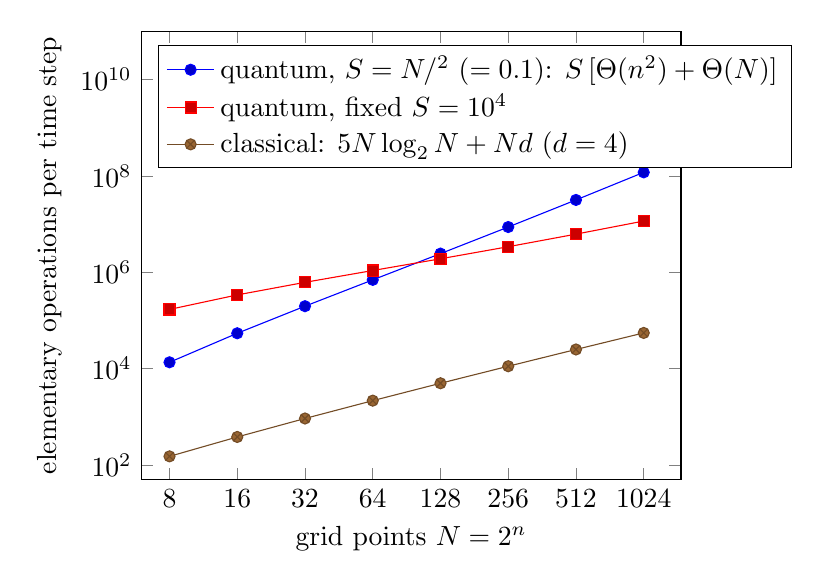
\begin{tikzpicture}
\begin{loglogaxis}[
  xlabel={grid points $N=2^{n}$},
  ylabel={elementary operations per time step},
  xmin=6,xmax=1500,ymin=50,ymax=1e11,
  xtick={8,16,32,64,128,256,512,1024},
  xticklabels={8,16,32,64,128,256,512,1024},
  legend pos=north west,
  legend cell align=left]
\addplot coordinates {(8,13600) (16,54400) (32,198400) (64,697600) (128,2444800) (256,8704000) (512,31744000) (1024,118681600)};
\addlegendentry{quantum, $S=N/\eps^{2}$ ($\eps=0.1$): $S\,[\Theta(n^{2})+\Theta(N)]$}
\addplot coordinates {(8,170000) (16,340000) (32,620000) (64,1090000) (128,1910000) (256,3400000) (512,6200000) (1024,11590000)};
\addlegendentry{quantum, fixed $S=10^{4}$}
\addplot coordinates {(8,152) (16,384) (32,928) (64,2176) (128,4992) (256,11264) (512,25088) (1024,55296)};
\addlegendentry{classical: $5N\log_2 N + Nd$ ($d=4$)}
\end{loglogaxis}
\end{tikzpicture}
\caption{Per-step cost of the hybrid quantum solver against the classical split-step solver as a function of grid size, evaluated from the cost model of \cref{eq:syn:costq,eq:syn:costc} with gate executions and floating-point operations placed on a common axis. Illustrative rendering of the model in \cite{guo2026nonlinearwaves}, not measured data; the slopes, not the absolute offsets, carry the conclusion.}
\label{fig:syn:cost}
\end{figure}

\subsection{What the Negative Result Means}\label{sec:syn:waves-meaning}

The direct route fails for a reason that has nothing to do with today's noise and everything to do with information. A nonlinear update needs $N$ numbers, and a quantum register does not release them for less than $\Theta(N)$ shots. Any proposal for end-to-end quantum advantage in nonlinear wave simulation must therefore contain a \emph{coherent} nonlinear update. Its cost per step must be $o(N)$ in gates and shots combined. The model of \cref{sec:syn:costmodel} gives the target concretely: match the $\Theta(n^{2})$ cost of the linear kernel, or at least beat $\Theta(N\log N)$ with a constant that survives the shot overhead of reading the final answer.

The linear-embedding routes can in principle meet this target for weakly nonlinear, dissipative problems~\cite{liu2021carleman}. The polynomial arithmetic on encoded states of \cref{ch:qml} (\nnqa{}) is a candidate primitive for the pointwise polynomial map in \cref{eq:syn:poly} without measurement. This chapter tells us how good such a primitive has to be. It also gives a template for honest accounting beyond fluids: whenever an algorithm's inner loop needs the data it is processing, count the read-out.

\section{Relation to the Other Chapters}\label{sec:syn:relation}

Both halves of this chapter rest on the HPC stack of \cref{ch:qgear}. \rubriq{} places \cudaq{} state-vector simulation inside a reinforcement-learning loop on Perlmutter, with the containers, Slurm integration and \qiskit{}-to-\cudaq{} lowering that \qgear{} provides. The nonlinear-wave study used GPU simulation to run the end-to-end hybrid solver at sizes beyond the hardware runs. The data-encoding family in the \rubriq{} benchmark and the reload step of the split-step solver are both \qcrank{}-type vectorized encoders. So the encoding work of \cref{ch:qml} supplies the loader whose $\Theta(N)$ cost \cref{eq:syn:costq} counts, and its \nnqa{} is the natural candidate for a coherent nonlinear update.

The T-count that \rubriq{} minimizes is the fault-tolerant cost defined by the error-correcting codes of \cref{ch:qec}. Its Clifford-fraction term is a tableau check in the stabilizer formalism that \cref{ch:qec} uses to build and audit encoders. Conversely, the seeded Clifford ensembles of \cref{ch:qec} are exactly the circuits that the Clifford term verifies at zero simulation cost. Finally, Part~B's cost discipline is to count shots, depth and reload latency, and to compare with the classical baseline at equal accuracy. The hardware-aware optimizers of \cref{ch:nisq} applied the same discipline to NISQ circuits, and this chapter carries it into the fault-tolerant setting.

\section{Summary}\label{sec:syn:summary}

This chapter answered RQ4 in two parts. Learned synthesis can produce circuits that respect fault-tolerant budgets when the learning signal is a dense, decomposable rubric evaluated at HPC scale. \rubriq{} fine-tunes a 7B coder with GRPO against a five-term rubric computed by \cudaq{} simulation on Perlmutter. On \num{1500} benchmark circuits it achieves $3.31\times$ mean T-gate compression against $2.05\times$ for sparse-reward RL, sub-$1\%$ hardware-constraint violations and $96\%$ correctness. It converges two to three times faster with proportionally fewer simulator calls, and its circuits were validated on IBM Heron~r3 and IonQ Forte~\cite{guo2026rubriq}.

Honest cost accounting was applied to the direct simulation of nonlinear waves. Reading the field at every step costs $\Theta(N^{2}/\eps^{2})$ gate executions per step against $\Theta(N\log N)$ classically, so no end-to-end advantage is possible without a coherent nonlinear update. The unified cost-and-error model, adaptive controller and hardware-validated kernels state that target quantitatively~\cite{guo2026nonlinearwaves}. The next chapter turns from the cost of fault-tolerant computation to whether it can be trusted on hardware the user does not own.
